\section{结果}
由于程序在图片过大、颜色位数过大时运行很慢($1080\times 1920\times 3$的24位真彩色图片要运行30分钟),所以在demo中我们以$512\times 512\times 3$的8位图片Lena为例进行了测试。
\begin{figure}[H]
	\centering
	\includegraphics[scale=0.4]{lena}
	\caption{Lena.}
	\label{lena}
\end{figure}

\subsection{小波变换结果分析}
选取第一个tile中的y分量分解得到的三级小波系数(这里以5/3 LG滤波器为例),将其按照\ref{fig5}所示的二维三级小波变换的区域划分进行排列。从图\ref{result1}中可以看到,第一级小波分解得到的LH,HL和HH分量中仍含有很多的图片纹理信息,而对LL分量进行进一步分解之后得到的二级和三级小波系数中纹理逐渐消失,说明信息得到了充分的分解。对于9/7 DB滤波器也有类似的结果。\textit{运行代码的时候将可选参数设为$debug=True$即可显示出小波系数可视化的图片。}
\begin{figure}[H]
	\centering
	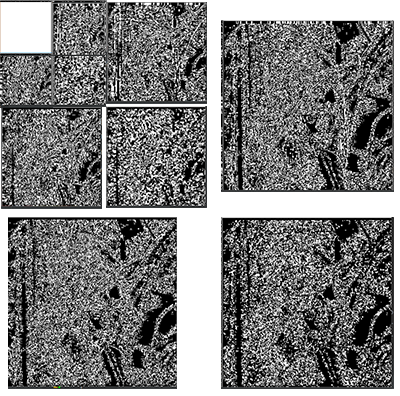
\includegraphics[scale=0.4]{result1}
	\caption{小波系数的可视化.}
	\label{result1}
\end{figure}

\subsection{压缩前后比较}
由生成压缩图像的大小来看,压缩效果并不理想,原因有二:\\
1. 需要存储的数据,绝大多数(除"图像"大小以外)都是在0-255的范围内,使用4个字节存储会有冗余。\\
2. 在解码时需要使用Context来估计0,1的概率分布,但是Context本身并不能直接反映图像内容。而且在一个block中,Context所占的字节数远大于Stream的字节数(我们也存储了只含有stream的二进制文件,比较两者的文件大小即可发现)。因此,\textbf{如何处理Context还需要进一步探究。}